\section{Radiation Protection during EDL}
\chapterauthor{Maja Tomicic}

As described in chapter \ref{chap:rad} the radiation environment around and on the surface of Europa is extreme. The protection of the payload from the radiation during the landing has been one of the main driving forces in the design of the landing module. The need for radiation shielding is conflicting with the need for minimizing the mass of the lander, and novel and creative designs have been necessary to accommodate both issues.


\subsection{Material}
Polyethene
Aluminum 
Titanium

\subsection{Radiation protection design}
To achieve the most mass efficient radiation shielding the payload is surrounded by a toroidal fuel tank. This design provides radiation shielding as a combination of shielding from the liquid propellant surrounding the payload and shielding by the tank aluminum walls. For mass considerations the inner wall surrounding the payload is thicker (7 mm) than the larger outer wall (2 mm). The design is illustrated in figure \ref{fig:tankdesign}.

\begin{figure}[htb]
\begin{center}
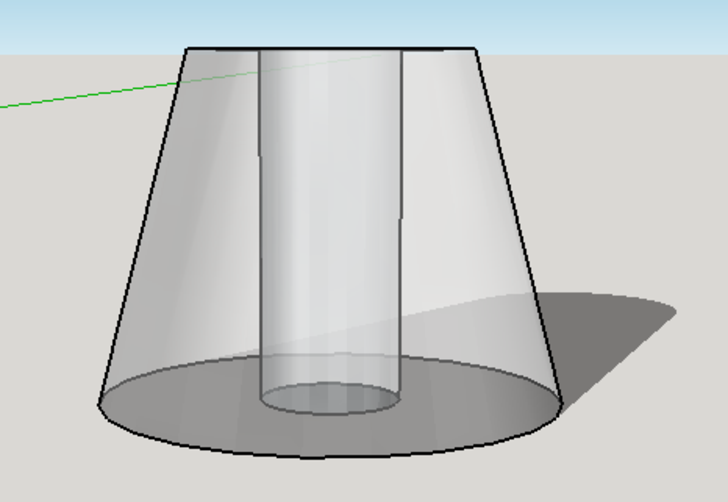
\includegraphics[scale=0.7]{figures/navtheory/tank}
\caption{Sketch of the tank design. The payload will be placed in the cylinder-shaped hole, thus being protected from the radiation by a combination of the liquid propellant and the aluminum walls of the tank. The inner wall surrounding the cylinder is thicker (7 mm) compared to the outer tank wall (2 mm). }
\label{fig:tankdesign}
\end{center}
\end{figure}

The main propellant stored in the tank will be liquid hydrazine N$_2$H$_4$. Materials rich in hydrogen and carbon are known to be effective shielding materials against energy radiation because they do not fragment into secondary particles as much as heavier elements when bombarded by high-energy radiation \cite{rad_shield_2006}. Thus the hydrazine will be an excellent radiation shield. 
However, the propellant will be consumed during the landing, thus not being efficient during the final part of the landing. Therefore the final radiation dose has been calculated as a worst case scenario where only the tank walls are considered. \\

Figure \ref{fig:raddose} shows the 2$\pi$ radiation dose in Rad/hour on the surface of Europa as a function of aluminum shielding thickness. 

\begin{figure}
\begin{center}
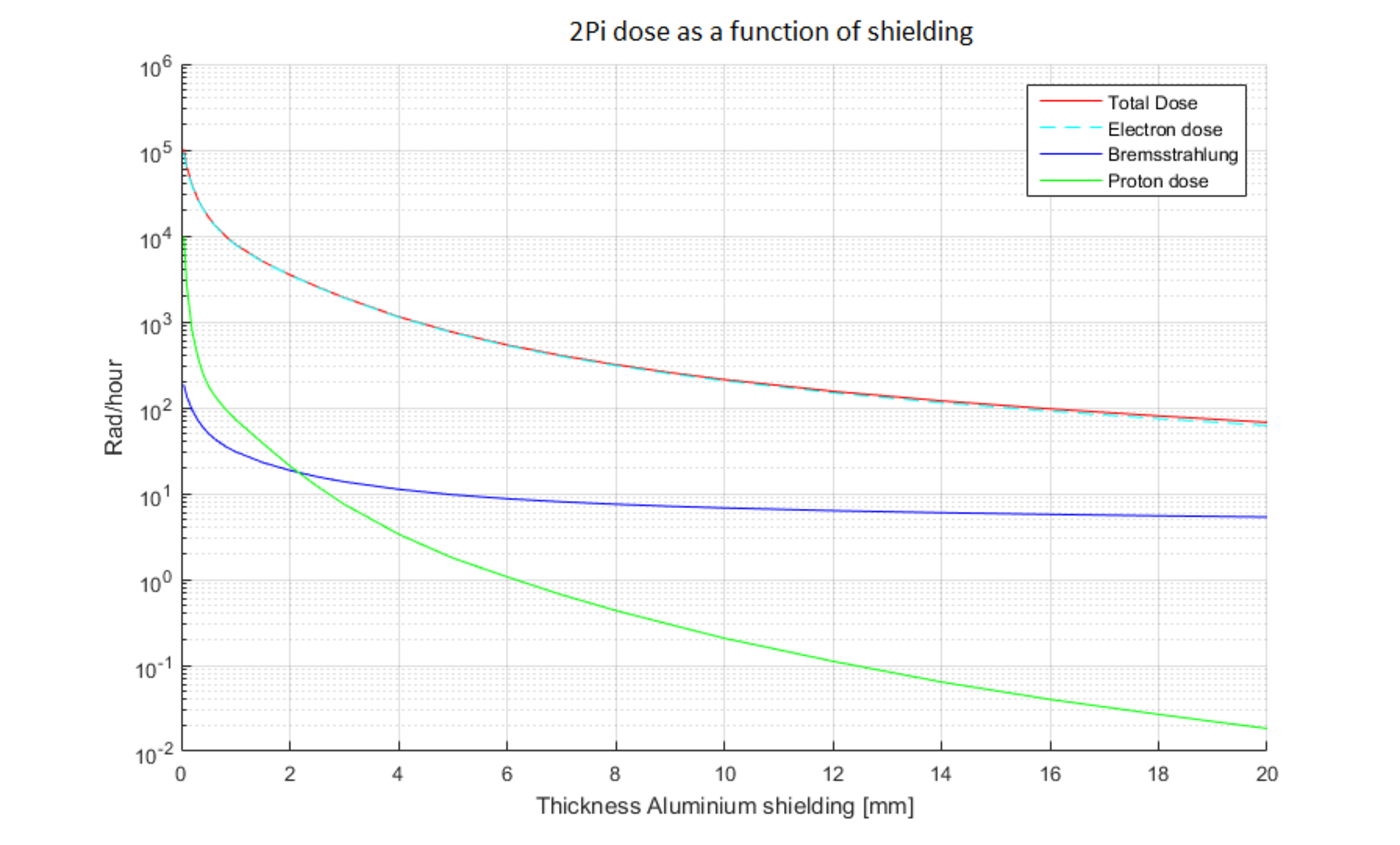
\includegraphics[scale=0.5]{figures/navtheory/dose}
\caption{Dose received on Europa in Rad/hour as a function of aluminum shield thickness. The graph is made with data from SPENVIS.}
\label{fig:raddose}
\end{center}
\end{figure}

